\chapter{Синтезирование голос}

Под термином "Синтезирование голоса" обычно понимается любой аудио-сигнал, важные характеристики которого были изменены при помощи технологий нейронных сетей, сохраняя при этом воспринимаемую естественность. Ранее проведенные исследования в основном выделяли пять видов дипфейкового звука:

\begin{enumerate}
    \item преобразование текста в речь;
    \item преобразование голоса; 
    \item подделка эмоций;
    \item подделка сцен;
    \item частично подделка.
\end{enumerate}

также в таблице (\ref{table::audio-class}), проведено классификация аудио дипфейков по способу генерации, где в первой столбце таблице представлены поддельные типы дипфейков, во второй столбце - поддельные черты, в третей столбце - поддельные продолжительности то есть частично или полностью синтезирован, в четвертом столбце - с помощью нейронной сети указывается что применяемый метод реализован ли с помощью нейронных сетей.

\section{Преобразование текста в речь}

Преобразование текста в речь (TTS) представляет собой широко применяемую технологию, ориентированную на синтез четкой и естественной речи из произвольного текста с использованием моделей, основанных на методах машинного обучения. Современные модели TTS в основном используют глубокие нейронные сети для генерации реалистичной речи, которая максимально приближена к человеческой.\\

Системы TTS обычно включают в себя два основных модуля: модуль анализа текста и модуль генерации речевых сигналов. Модуль анализа текста разбирает входной текст, определяя тон, интонацию и другие лингвистические аспекты, необходимые для правильной передачи смысла. Затем модуль генерации речевых сигналов создает звуковую последовательность, соответствующую заданному тексту.

\section{Преобразование голоса} 

Преобразование голоса (VC) [8], или клонирование голоса в цифровой форме, фокусируется на изменении звучания речи одного говорящего, подражая тембру и просодии другого говорящего, при этом сохраняя содержание оригинального высказывания. Процесс введения в систему VC обычно включает в себя использование естественных высказываний данного говорящего как входных данных.\\

Существует несколько основных подходов к технологиям VC [18], включая статистический параметрический, частотное искажение и выбор единиц измерения. В частности, статистическая параметрическая модель включает в себя вокодер, аналогичный тому, который используется в статистических параметрических системах синтеза речи (TTS).
\section{Подделка эмоций}


Подделка эмоций [25], также известная как модификация эмоционального тонуса, представляет собой технологию, направленную на изменение акустических характеристик звука с целью создания впечатления изменения эмоционального состояния говорящего. Эта методика фокусируется на манипуляции параметрами, такими как тембр, интонация и темп речи, сохраняя при этом остальные аспекты звуковой информации, такие как личность говорящего и содержание высказывания.

\section{Подделка сцен}

Модификация сцены звучания, более известная как подделка сцены [27], представляет собой метод, направленный на сопоставление акустической обстановки оригинального высказывания с другой звуковой сценой, используя технологии улучшения речи. В этом процессе сохраняются как личность говорящего, так и содержание высказывания, при этом происходит изменение окружающей аудиообстановки.

\section{Частично подделка}

Частичная подделка [28], также известная как модификация части высказывания, представляет собой технику, прицельно изменяющую всего лишь несколько слов в оригинальном высказывании. Этот метод осуществляется путем манипулирования исходными аудиоклипами с использованием подлинных или созданных синтезом звуковых фрагментов. Однако при этом ключевым аспектом является сохранение неизменной личности говорящего.

\begin{table}[H]
	\centering
	\setlength{\tabcolsep}{8pt} % Adjust column spacing
	\renewcommand{\arraystretch}{1.3} % Adjust row spacing
    \caption{Класификации аудио дипфейков по способу генерации}\label{tab:class}
    \captionsetup{justification=raggedright,singlelinecheck=false}
    \begin{tabular}{|p{4cm}|p{3cm}|p{3cm}|p{3cm}|}	
        \hline
		\thead{Поддельный тип} & \thead{Поддельная черта} & \thead{Поддельная продолжительность}  & \thead{С помощью нейронной сети}  \\ 
		\hline
		Преобразование  текста в речь    & Личность спикера, Речевое содержание  & полностью	  	 &  да  \\
		\hline
		Преобразование голоса   & Личность спикера & полностью  &  да \\
		\hline
		Подделка эмоций & эмоция спикера 	& полностью  &  да \\
		\hline
		Подделка сцен  & Акустическая сцена & полностью  &  да \\
		\hline
		Частично подделка  & Речевое содержание 	& частично  &  да \\
		\hline
    \end{tabular}
    \label{table::audio-class}
\end{table}

\chapter{Отличительные признаки аудио для изучения}

Извлечение признаков представляет собой ключевой модуль классификатора аудиодипфейков. Основной целью этого процесса является изучение характерных особенностей путем выделения акустических артефактов из речевых сигналов, которые могут свидетельствовать о наличии поддельных атак. Большое количество исследований подчеркнуло важность определения полезных признаков для эффективного обнаружения дипфейков.

В данной области уделено значительное внимание выявлению полезных функций, способных обнаруживать характерные аспекты поддельных атак. Признаки, использованные в проведенных исследованиях, условно могут быть разделены на три основные категории [48]: 

\begin{itemize}
    \item Спектральные особенности;
    \item Просодические особенности;
    \item Глубокие особенности.
\end{itemize}

\section{Спектральные особенности}

Спектральные характеристики в анализе звука относятся к характеристикам, которые отражают распределение энергии по различным частотам в сигнале. Эти характеристики вычисляются с использованием математических преобразований, таких как быстрое преобразование Фурье (FFT), и имеют критическое значение для извлечения существенной информации из аудиосигналов для различных применений. Спектральные характеристики могут быть классифицированы на краткосрочные и долгосрочные в зависимости от временного масштаба, в течение которого они вычисляются.

\subsection{Кратковременные спектральные особенности}

Кратковременные спектральные характеристики, извлеченные из коротких кадров обычно длительностью 20-30 мс, описывают кратковременную спектральную огибающую, которая включает в себя акустический коррелят тембра голоса. Кратковременные спектральные характеристики вычисляются, главным образом, путем применения кратковременного преобразования Фурье (STFT) к речевому сигналу [52]. При предположении, что речевой сигнал x(t) квазистационарен в течение короткого периода, STFT формулируется следующим образом:


\begin{equation}
    X(t, \omega) = |X(t, \omega)| e^{j\phi(\omega)}
\end{equation}

где \(|X(t, \omega)|\), это спектр магнитуд а \(\phi(\omega)\) представляет собой фазовый спектр в кадре t и частотный диапазон \(\omega\). Спектр мощности определяется как \(|X(t, \omega)|^2\).

Кратковременные спектральные характеристики в основном включают кратковременные характеристики, основанные на магнитуде и фазе. Обычно несколько характеристик, базирующихся на магнитуде, напрямую производятся из спектра магнитуды, но большинство из них вычисляются из спектра мощности. Характеристики, основанные на фазе, извлекаются из фазового спектра.

Спектр магнитуды представляет собой график амплитуд сигнала в зависимости от его частоты, тогда как спектр мощности включает в себя квадрат амплитуд, отражающий распределение энергии. Кратковременные характеристики, основанные на магнитуде, могут включать в себя параметры, такие как частоты формант, амплитудные спектральные величины и мел-частотные кепстральные коэффициенты (MFCC).

Характеристики, вычисленные на основе фазы, включают в себя информацию о временных задержках и относительных фазовых сдвигах между различными частотами. Эти параметры могут быть полезными при анализе изменений во времени и при восстановлении оригинального сигнала.

\subsection{Долгосрочные спектральные особенности}

Кратковременные спектральные признаки не очень хорошо передают временные характеристики траекторий речевых признаков из-за того, что они вычисляются покадрово [60]. Поэтому были предложены долгосрочные спектральные характеристики для получения информации на более широких временных интервалах из речевых сигналов, и исследования показали, что они имеют решающее значение для обнаружения поддельной речи.

Долгосрочные спектральные характеристики охватывают более продолжительные временные участки речевых сигналов и могут лучше отражать долгосрочные изменения в акустических свойствах речи. Это позволяет системе обнаружения более эффективно анализировать речевые траектории и выявлять особенности, связанные с поддельной речью. Такие характеристики могут включать в себя долгосрочные форманты, изменения в спектральной энергии на протяжении времени и другие параметры, охватывающие более широкие аспекты речевого сигнала [49].

\section{Просодические особенности}

Просодия относится к несегментарной информации в речевых сигналах, включая ударение на слоге, интонационные паттерны, темп речи и ритм [78]. В отличие от кратковременных спектральных характеристик с короткой продолжительностью, обычно составляющей 20-30 мс, просодические особенности охватывают более длинные сегменты, такие как фоны, слоги, слова, высказывания и т.д. Важные просодические параметры включают основную частоту (F0), длительность, распределение энергии, скорость разговора и т.д. Предыдущие исследования [78] по обнаружению поддельного звука в основном рассматривали три основные просодические характеристики:

\begin{itemize}
    \item Основная частота (F0): Показатель высоты голоса, который варьируется в зависимости от интонации и эмоционального состояния говорящего;
    \item Длительность: Временной параметр, отражающий продолжительность звуковых сегментов, таких как слоги и слова, в речевом потоке;
    \item Распределение энергии: Характеризует энергетические аспекты речи и может отражать эмфатическое выделение или особенности интонации.
\end{itemize}

Эти просодические характеристики могут быть использованы для выделения особенностей в произношении, что делает их важными для обнаружения поддельного звука, где подделка может влиять на натуральные просодические паттерны голоса. Однако они менее чувствительны к канальным эффектам по сравнению со спектральными функциями [8]. Они могут предоставлять дополнительную информацию к спектральным функциям для повышения эффективности обнаружения поддельного звука.

\section{Глубокие особенности}

Упомянутые выше спектральные особенности и просодические характеристики представляют собой большую часть ручных функций с сильными и желательными репрезентативными способностями. Однако их конструирование подвержено предвзятостям из-за ограничений представлений, внесенных человеческими разработчиками [51]. Таким образом, глубокие функции вдохновлены для заполнения этого пробела. Глубокие функции изучаются с использованием глубоких нейронных сетей, которые условно можно разделить на три категории: обучаемые спектральные функции, контролируемые функции встраивания и самоконтролируемые функции встраивания.

На рисунке (\ref{fig:audio-classification}) представлено, класификации аудио по признаками для обучение: 
\begin{figure}[H]
	\centering
	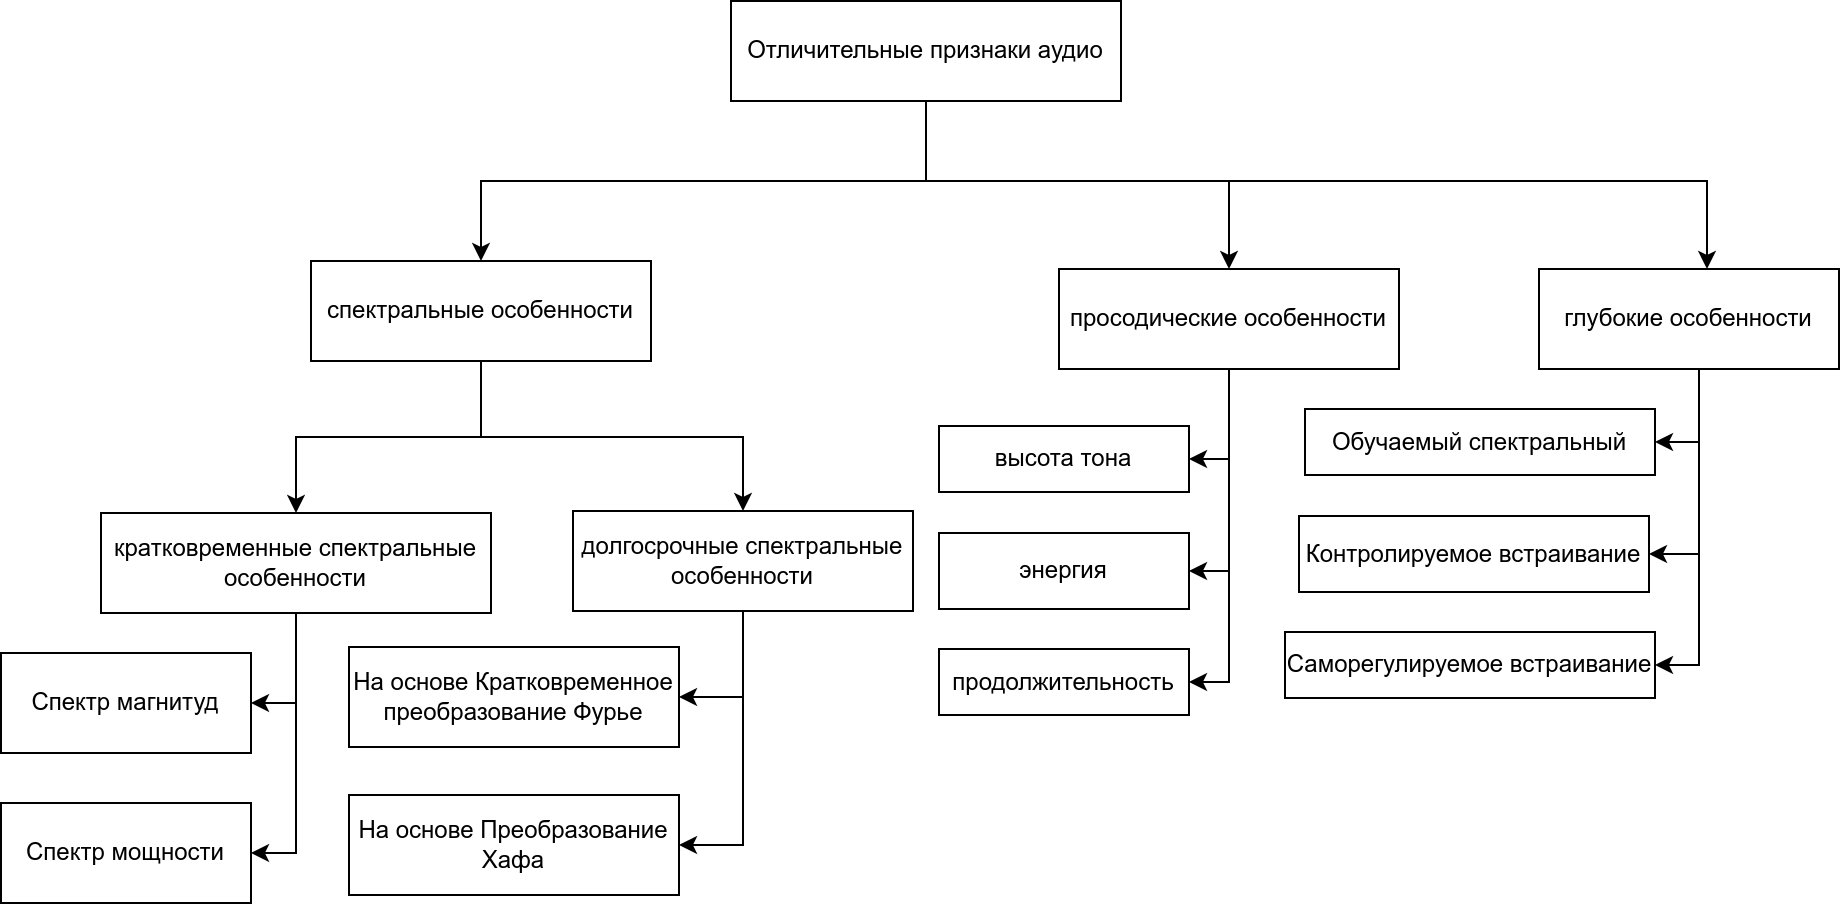
\includegraphics[width=0.9\linewidth]{images/classification-of-audio.png}
	\caption{Классификации аудио по признаками}
	\label{fig:audio-classification}
\end{figure}


\chapter{Система обнаружения поддельного звука (англ. Audio deepfake detector)}

В системах, используемых для обнаружения поддельного звука, важным фактором являются аудио-особенности для изучения, и внутренний классификатор играет ключевую роль в глубоком распознавании аудио. Целью является изучение высокоуровневого представления функций входного интерфейса и моделирование превосходных возможностей обнаружения. Внутренние классификаторы, которые часто используются для обнаружения аудио-дипфейков, в основном делятся на две категории:
\begin{itemize}
    \item Статистические методы;
    \item С использованием глубоких нейронных сетей.
\end{itemize}

\section{Статистические методы обнаружения Аудио Дипфейк}

Под термином "статистические методы" в статьях часто подразумевают алгоритмы машинного обучения, которые изучают характеристики аудио для решения задачи обнаружения аудио-дипфейков. Для этого используются алгоритмы бинарной классификации.

В связи с этим для обнаружения фальшивой речи было использовано множество классических подходов к классификации паттернов. Самые популярные методы обнаружения аудио-дипфейков с применением машинного обучения включают:

\begin{itemize}
    \item Машина опорных векторов (англ. Support Vector Machine);
    \item Гауссовые моделей смеси (англ. Gaussian mixture model).
\end{itemize}

\subsection{Машина опорных векторов (SVM)}

SVM - это контролируемый метод обучения, который основывается в основном на двух предположениях \cite{hamza2022deepfake}:
\begin{enumerate}
    \item Преобразование данных в многомерное пространство может свести сложные проблемы классификации со сложными поверхностями принятия решений к более мелким проблемам, которые могут быть решены путем их линейного разделения;
    \item Только обучающие шаблоны вблизи поверхности принятия решений обеспечивают наиболее чувствительную детали для классификации.
\end{enumerate}

Так как, проблема обнаружения аудио дипфейков представляет собой бинарную классификацию с линейно разделяемыми векторами \(x_{i} \in \mathbb{R}^{n}\), в качестве поверхности принятия решения, используемой для классификации паттерна как принадлежащего к одному из двух классов, используется гиперплоскость \(H_{0}\). Если х это случайный вектор n * \(\mathbb{R}\), тогда мы определяем:

\begin{equation}
    f_{(x)} = w.x + b
\end{equation}

В формуле (.) это скалярное произведение, набор всех x-векторов, удовлетворяющих уравнению \(f_{(x)} = 0\), обозначается как \(H_{0}\). Предполагая две гиперплоскости, \(H_{1}\) и \(H_{2}\), расстояние между ними называется их границей, которую можно представить следующим образом:

\begin{equation}
    \begin{cases}
        H_{1} = \{x \in \mathbb{R}^{n} | f_{(x)} > 0\} \\
        H_{2} = \{x \in \mathbb{R}^{n} | f_{(x)} < 0\}
    \end{cases}
\end{equation}

Гиперплоскость решения \(H_{0}\) зависит от векторов, ближайших к двум параллельным гиперплоскостям, называемым опорными векторами. Запас должен быть максимальным, чтобы получить классификатор, который не очень адаптирован к обучающим данным.

На рисунке (\ref{fig:support-vector-machine}) представлено, машина опорных векторов: 
\begin{figure}[H]
	\centering
	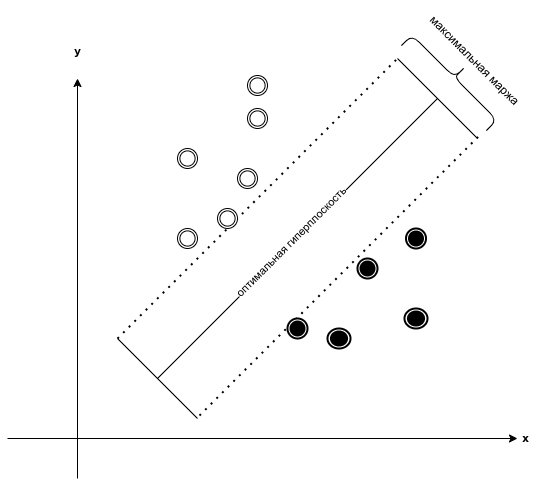
\includegraphics[width=0.4\linewidth]{images/support-vector-machine.png}
	\caption{Машина опорных векторов (SVM)}
	\label{fig:support-vector-machine}
\end{figure}

В многих статьях по классификации аудио-дипфейков где классификатор реализован на базе SVM. SVM отлично справляется с четким разделением выборок и эффективен в средах с высокой размерностью. SVM использует подмножество точек обучения в функции принятия решения, что делает его эффективным с точки зрения использования памяти.

% \subsubsection*{Методы с применением SVM}
% 
% В статей [110] и [68], используют машина опорных векторов в качестве классификатора, в статей [110] предполагают, что классификаторы SVM по своей сути устойчивы к атакам с искусственным подменой сигналов. Однако очень трудно определить точную природу атак с подменой в практических сценариях.
% В статей [68] предложили одноклассовый классификатор SVM, обученный только использованию подлинных высказываний для классификации реальных и поддельных голосов, который хорошо подходит для неизвестных атак с использованием подделки.

\subsection{Гауссовые моделей смеси (GMM)}

Модель гауссовой смеси (GMM), как следует из названия, представляет собой смесь нескольких гауссовых распределений. Речевые признаки представлены в виде векторов в n-мерном пространстве. Распределение этих векторов признаков представлено смесью гауссовых плотностей. \\ Для n-мерного вектора признаков \(x\) функция плотности смеси для класса \(s\) с параметром модели \(\lambda^{s}\) определяется как \cite{JOTHILAKSHMI2016301}:

\begin{equation}
    p(x | \lambda^{s}) = \sum_{i = 1}^{\mathcal{M}} \alpha^{s}_{i} f_{i}^{s}(x)
\end{equation}

Функция плотности смеси представляет собой взвешенную линейную комбинацию \mathcal {M} унимодальных гауссовых плотностей компонентов \(f_ {i}^{s}(.)\). Каждая функция гауссовой плотности \(f_{i}^{s}(.)\) параметризуется вектором среднего \(\mu_{i}^{s}\) и ковариационной матрицей \(\Sigma_{i}^{s}\) с использованием:

\begin{equation}
    f_{i}^{s}(x) = \frac{1}{\sqrt{(2\pi)^{n}|\Sigma_{i}^{s}|}} \exp \left(-\frac{1}{2}(x - \mu_{i}^{s})^T \Sigma_{i}^{s}^{-1} (x - \mu_{i}^{s})\right)
\end{equation}

где \(\Sigma_{i}^{s}\) является ковариационной матрией и \((\Sigma_{i}^{s})^{-1}\) называется обратной ковариационной матрией.

% \subsubsection*{Методы с применением GMM}
% 
% В статей [32] и [114], в качестве классификатора используется GMM. в статей [32] используется в качестве классификатора человеческих и синтезированных голосов.
% в статей [114], предложят метод, который определяет разницу между реальной и преобразованной речью, используя логарифмическое отношение правдоподобия, основанное на модели GMM для реальной и преобразованной речи.

\section{Методы с применением глубоких нейронных сетей}

Классификаторы современных систем обнаружения аудио-дипфейков в основном основаны на методах глубокого обучения, которые значительно превосходят классификаторы, основанные на SVM и GMM, благодаря их мощным возможностям моделирования [145]. 

Каждый аудиосигнал может быть представлен на двумерном графике, построенном с использованием математических расчетов. Обработка аудиозаписей в нейронной сети требует большого объема вычислений для создания системы, способной обнаруживать аудио-дипфейки с гораздо меньшими затратами вычислений. Это достигается путем преобразования аудиозаписей в изображения звуковых объектов и последующего получения значений массива в числовом формате, наилучшим образом подходящих для передачи в качестве входных данных в нейронную сеть. 

Существует соревнование научных статей по созданию и обнаружению синтезированного звука под именем ASVSpoof \cite{yamagishi2021asvspoof}. В этом соревновании предлагаются три метода применения глубоких нейронных сетей для обнаружения синтетического звука:

% \begin{enumerate}
%     \item 
% \end{enumerate}
% \subsection{Сверточные нейронные сети}
% Компьютерное зрение - увлекательная тема, на сегодняшний день является одним из часто применением методов для изучение и анализа изображении.
% Сверточные нейронные сети играет важнешей роль в задачах компьютерное зрение, главным фактором в сверточных нейронных сетях является фелтеры.
% Эти фильтры представляют собой скользящие окна, которые отвечают за обнаружение особенностей или паттернов на изображении.